\section{Introduction to Space Complexity}

So far, we have focused on \textbf{time complexity}. Today, we will explore \textbf{space complexity}, which measures the memory resources
an algorithm uses. Space complexity is important for two key reasons:

\begin{enumerate}
    \item It quantifies the \textbf{memory consumption} of an algorithm.
    \item If two algorithms have the \textbf{same time complexity}, but one uses more space, the latter may run slower due to higher memory overhead.
\end{enumerate}

We will only consider space complexity for \textbf{decidable Turing Machines (TMs)}, meaning they halt on all inputs. 
With this in mind, let's formally define space complexity.

\section{Space Complexity Definitions}

\subsection{1. Deterministic Turing Machines (DTM)}
The \textbf{space complexity} of a decidable deterministic TM is a function \( f: \mathbb{N} \rightarrow \mathbb{N} \), where \( f(n) \) is 
the \textbf{maximum number of tape cells visited} by the TM on any input of size \( n \).

\subsection{2. Non-Deterministic Turing Machines (NTM)}
The \textbf{space complexity} of a decidable non-deterministic TM is a function \( f: \mathbb{N} \rightarrow \mathbb{N} \), 
where \( f(n) \) is the \textbf{maximum number of tape cells visited} by the TM \textbf{along any computational branch} for any input of size \( n \).

\section{Clarifying the Notion of ``Visited'' in Space Complexity}

To properly analyze space complexity, we must precisely define what constitutes a ``visited'' tape cell:

\begin{definition}[Visited Cell]
A tape cell is considered \textbf{visited} if the Turing Machine's read/write head ever occupies or scans that cell during computation. Each distinct cell visited contributes exactly one unit to the space complexity, regardless of how many times it is accessed.
\end{definition}

\subsection{Contrast with Time Complexity}
\begin{itemize}
    \item \textbf{Space Complexity} counts only the \textit{number of distinct cells} ever accessed during computation. Multiple accesses to the same cell do not increase the space measure.

    \item \textbf{Time Complexity} counts the \textit{total number of transitions} executed by the TM. Each basic operation (read, write, move, state change) constitutes one transition, regardless of whether it involves previously accessed cells.

%    \item \textbf{Configuration vs Transition}: While a configuration (complete state snapshot including tape contents, head position, and control state) is useful for decidability proofs, time complexity specifically counts transitions between configurations.
\end{itemize}

\subsection{Key Implications}
\begin{itemize}
    \item Space complexity depends only on the \textit{maximum workspace} needed, not on how frequently cells are reused.

    \item Time complexity depends on the \textit{total computation length}, counting every transition, including repeated operations on the same cells.

    \item This distinction explains why some problems can have different space and time complexity classes (e.g., problems in $\text{PSPACE}$ but not $\text{P}$).
\end{itemize}

\begin{example}
Consider a TM that writes $n$ bits by repeatedly moving back-and-forth across $O(1)$ cells:
\begin{itemize}
    \item Its \textit{space complexity} is $O(1)$ (fixed number of cells)
    \item Its \textit{time complexity} is $\Omega(n)$ ($n$ transitions needed)
\end{itemize}
\end{example}


\section{Complexity Classes for Space}

We now define some fundamental classes of space complexity:

\subsection{SPACE(\( f(n) \))}
\[
\text{SPACE}(f(n)) = \{ B \mid \text{some deterministic 1-tape TM } M \text{ decides } B \text{ using } O(f(n)) \text{ space} \}
\]
A more precise name for this class is \textbf{DSPACE(\( f(n) \))}, but we will use the conventional notation.

\subsection{NSPACE(\( f(n) \))}
\[
\text{NSPACE}(f(n)) = \{ B \mid \text{some non-deterministic 1-tape TM } M \text{ decides } B \text{ using } O(f(n)) \text{ space} \}
\]

\subsection{PSPACE}
\[
\text{PSPACE} = \bigcup_{k \in \mathbb{N}} \text{SPACE}(n^k)
\]
Thus, PSPACE contains all languages decidable by a deterministic TM using \textbf{polynomial space}.

\subsection{NPSPACE}
\[
\text{NPSPACE} = \bigcup_{k \in \mathbb{N}} \text{NSPACE}(n^k)
\]
Thus, NPSPACE contains all languages decidable by a non-deterministic TM using \textbf{polynomial space}.

These classes help us categorize problems based on their \textbf{memory requirements} under deterministic and non-deterministic computation models.

\section{Space Complexity of Multitape Turing Machines}

\begin{definition}
For a $k$-tape Turing machine $M$, its \textbf{space complexity} is the function $f: \mathbb{N} \rightarrow \mathbb{N}$ where $f(n)$ represents the 
maximum total number of distinct cells visited across \emph{all} tapes during $M$'s computation on any input of length $n$. 
\end{definition}

\begin{theorem}[Multitape to Single-Tape Simulation]
    Any $k$-tape Turing machine (TM) with space complexity $O(s(n))$ can be simulated by a single-tape TM with the same space complexity, 
    i.e., $O(s(n))$, with the space only increased by a constant factor. 
    This constant factor depends only on the number of tapes $k$, and not on the input size $n$.
\end{theorem}

    
\section{Relationship Between Time and Space Complexity}

\begin{theorem}[Time-Space Containment]
    For any space-constructible function $t(n) \geq n$:
    \begin{enumerate}
        \item $\text{TIME}(t(n)) \subseteq \text{SPACE}(t(n))$ \\
        (A machine using $t(n)$ time can visit at most $t(n)$ tape cells, hence its space usage is bounded by $t(n)$.)
        
        \item $\text{SPACE}(t(n)) \subseteq \text{TIME}(2^{O(t(n))})$ \\
        (A machine using $t(n)$ space has at most $2^{O(t(n))}$ possible configurations, so it must halt within that many transitions if it halts at all.)
    
        \item Based on the first inclusion, we can conclude that:
        \begin{itemize}
            \item $P \subseteq PSPACE$
            \item $EXPTIME \subseteq EXPSPACE$
            \item $NP \subseteq NPSPACE$
        \end{itemize}
    
        \item Based on the second inclusion, we can conclude that:
        \begin{itemize}
            \item $PSPACE \subseteq EXPTIME$
            \item $NPSPACE \subseteq EXPTIME$ \\
            (Because by Savitch’s theorem, $NPSPACE = PSPACE$, so the same time bound applies.)
        \end{itemize}
    \end{enumerate}    
\end{theorem}

\subsection{Explanation of the Containments}

\begin{description}
    \item[Time Bounds Space:] 
    Each transition of a TM can access at most one new tape cell. Therefore, a machine that halts after $O(t(n))$ transitions cannot use more than $O(t(n))$ space:
    \[
    \text{TIME}(t(n)) \subseteq \text{SPACE}(t(n))
    \]
    
    \item[Space Bounds Time via Configurations:]
    For a TM using $O(t(n))$ space:
    \begin{itemize}
        \item Let $Q$ be the set of states ($|Q|$ constant)
        \item Let $\Gamma$ be the tape alphabet ($|\Gamma|$ constant)
        \item Number of head positions: $O(t(n))$
        \item Number of possible tape contents: $|\Gamma|^{O(t(n))} = 2^{O(t(n))}$
    \end{itemize}
    Thus, the total number of distinct configurations is:
    \[
    |Q| \times O(t(n)) \times 2^{O(t(n))} = 2^{O(t(n))}
    \]
    
    Since the machine must halt (by decidability), it cannot execute more transitions than its number of possible configurations (otherwise it would repeat a configuration and loop forever). Therefore:
    \[
    \text{SPACE}(t(n)) \subseteq \text{TIME}(2^{O(t(n))})
    \]
\end{description}

\subsection{Key Observations}
\begin{itemize}
    \item Each transition corresponds to one unit of time complexity
    \item The configuration count ($2^{O(t(n))}$) provides an upper bound on possible distinct transitions before halting
    \item This explains why $\text{PSPACE} \subseteq \text{EXP}$ (problems solvable in polynomial space can require exponential time)
\end{itemize}

\section{Relationship Between NP and PSPACE}

\begin{theorem}
    $NP \subseteq PSPACE$
\end{theorem}

\begin{proof}
The proof proceeds in the following steps:
\begin{enumerate}
    \item \textbf{Proof that $SAT \in PSPACE$:}  
    Although $SAT$ is an NP-complete problem, it can be decided using polynomial space by trying all possible truth assignments sequentially without storing all of them simultaneously. We can evaluate each assignment one-by-one using only polynomial space, because storing a single assignment and checking the formula can be done within space proportional to the input size.

    \item \textbf{Proof that if $A \le_p B$ and $B \in PSPACE$, then $A \in PSPACE$:}  
    Suppose $f$ is a polynomial-time reduction from $A$ to $B$, and we have a polynomial-space algorithm for $B$. To decide if $x \in A$, we compute $f(x)$ (which requires only polynomial time, and hence polynomial space), and then decide whether $f(x) \in B$ using the polynomial-space algorithm for $B$. Thus, $A$ can be decided in polynomial space.

    \item \textbf{Conclusion:}  
    Every language $L \in NP$ is polynomial-time reducible to $SAT$ (since $SAT$ is NP-complete). By steps 1 and 2, and since polynomial-time reductions preserve membership in $PSPACE$, we conclude that $L \in PSPACE$. Hence, $NP \subseteq PSPACE$.
\end{enumerate}
\end{proof}

\begin{theorem} $PSPACE = coPSPACE$\end{theorem}
\begin{proof}
    \subsection{Closure Under Complementation}

\begin{theorem}[PSPACE = coPSPACE]
The complexity class PSPACE is closed under complementation. That is:
\[
\text{PSPACE} = \text{coPSPACE}
\]
\end{theorem}

\begin{proof}[Proof Sketch]
For any language $L \in \text{PSPACE}$, let $M$ be a TM that decides $L$ using polynomial space. We can construct a machine $M'$ that decides $\overline{L}$ (the complement of $L$) as follows:

\begin{enumerate}
    \item $M'$ simulates $M$ using the same polynomial space bound $p(n)$
    \item When $M$ would accept, $M'$ rejects
    \item When $M$ would reject, $M'$ accepts
    \item $M'$ maintains the same space complexity since:
    \begin{itemize}
        \item It uses exactly the same tape cells as $M$
        \item The finite control only needs constant additional space to track the inverted acceptance condition
    \end{itemize}
\end{enumerate}

The key observations are:
\begin{itemize}
    \item Space-bounded computation can be \textit{deterministically} complemented without increasing space usage
    \item Unlike time complexity, we don't need to worry about "timing out" - the space bound guarantees termination
    \item This fails for nondeterministic space classes unless Savitch's theorem gives us determinization (which it does for polynomial space)
\end{itemize}
\end{proof}

\paragraph{Contrast with Other Complexity Classes}
\begin{itemize}
    \item \textbf{Time Classes:} $\text{P} = \text{coP}$ (by similar argument), but it remains unknown whether $\text{NP} = \text{coNP}$
    \item \textbf{Logarithmic Space:} $\text{L} = \text{coL}$ (by Szelepcsényi's theorem for NSPACE)
    \item \textbf{General Pattern:} Space-bounded classes tend to be closed under complementation, while time-bounded classes may not be
\end{itemize}

\paragraph{Significance}
This property demonstrates an important advantage of space-bounded computation:
\begin{itemize}
    \item Space resources can be \textit{reused} during computation
    \item There's no need to store computation history for complementation
    \item Contrast with time-bounded computation where complementation might require storing or recomputing information
\end{itemize}
\end{proof}

\begin{theorem}
    $coNP \subseteq PSPACE$
\end{theorem}

\begin{proof}
The proof proceeds as follows:
\begin{enumerate}
    \item \textbf{Fact:} It is known that $PSPACE = coPSPACE$, meaning the class of languages decidable in polynomial space is closed under 
    complementation.

    \item \textbf{Conclusion:}  
    Since $NP \subseteq PSPACE$, taking complements yields $coNP \subseteq coPSPACE = PSPACE$.
\end{enumerate}
\end{proof}

\section{Open Problems in Space Complexity}

Space complexity theory contains several fundamental unresolved questions. Below we present the most significant open problems with their current status.

Although we know that $\mathbf{NP}, \mathbf{coNP} \subseteq \mathbf{PSPACE}$, it is still unknown whether $\mathbf{NP} = \mathbf{coNP}$ or whether either of them equals $\mathbf{P}$. These inclusions help structure the complexity landscape, as illustrated in the diagram below.

\begin{center}
    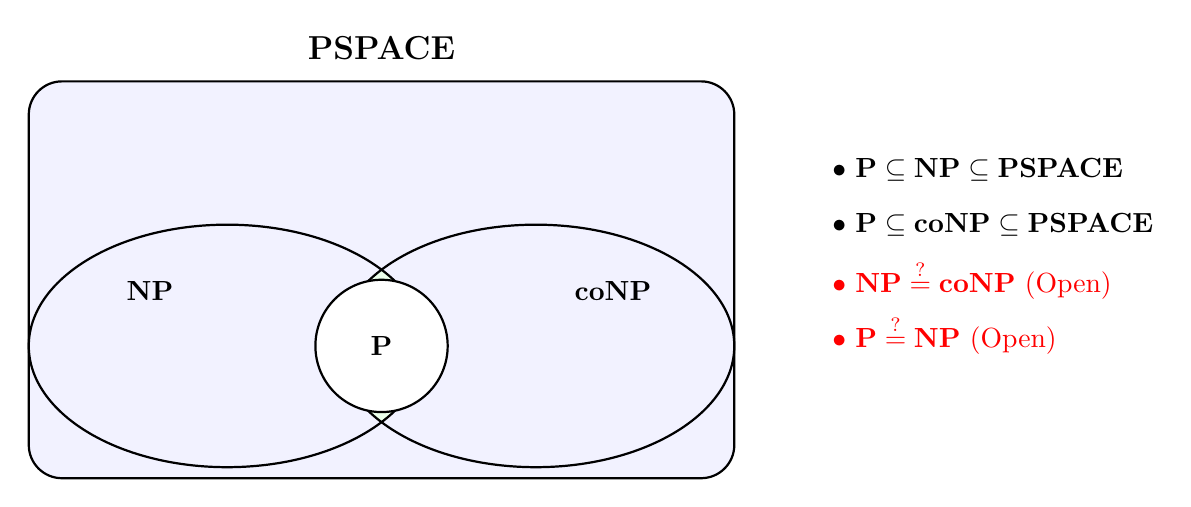
\begin{tikzpicture}[scale=1.4]
      % PSPACE - largest container
      \draw[thick, rounded corners=12pt, fill=blue!5] (-3.2,-1.8) rectangle (3.2,1.8);
      \node at (0,2.1) {\large\textbf{PSPACE}};
      
      % NP and coNP - properly contained intersecting ellipses
      \begin{scope}
        \clip (-1.4,-0.6) ellipse (1.8cm and 1.1cm);
        \fill[green!8] (1.4,-0.6) ellipse (1.8cm and 1.1cm);
      \end{scope}
      \draw[thick] (-1.4,-0.6) ellipse (1.8cm and 1.1cm);
      \draw[thick] (1.4,-0.6) ellipse (1.8cm and 1.1cm);
      \node at (-2.1,-0.1) {\textbf{NP}};
      \node at (2.1,-0.1) {\textbf{coNP}};
      
      % P - smallest circle in the intersection
      \draw[thick, fill=white] (0,-0.6) circle (0.6cm);
      \node at (0,-0.6) {\textbf{P}};
      
      % Right-side text explanations
      \node[align=left, anchor=west] at (4,1.0) {$\bullet\ \mathbf{P} \subseteq \mathbf{NP} \subseteq \mathbf{PSPACE}$};
      \node[align=left, anchor=west] at (4,0.5) {$\bullet\ \mathbf{P} \subseteq \mathbf{coNP} \subseteq \mathbf{PSPACE}$};
      \node[align=left, anchor=west,red] at (4,0.0) {$\bullet\ \mathbf{NP} \stackrel{?}{=} \mathbf{coNP}$ (Open)};
      \node[align=left, anchor=west,red] at (4,-0.5) {$\bullet\ \mathbf{P} \stackrel{?}{=} \mathbf{NP}$ (Open)};
    \end{tikzpicture}
\end{center}

\subsection{Class Containment Problems}

\begin{itemize}
    \item \textbf{$\mathbf{P}$ vs $\mathbf{PSPACE}$}
    \begin{itemize}
        \item[\textit{Known}:] $\mathbf{P} \subseteq \mathbf{PSPACE}$ (via space-time hierarchy)
        \item[\textit{Open}:] Is the containment proper?
        \item[\textit{Significance}:] Would imply all polynomial-space algorithms can be made time-efficient
        \item[\textit{Conjecture}:] $\mathbf{P} \neq \mathbf{PSPACE}$
    \end{itemize}

    \item \textbf{$\mathbf{NP}$ vs $\mathbf{PSPACE}$}
    \begin{itemize}
        \item[\textit{Known}:] $\mathbf{NP} \subseteq \mathbf{PSPACE} \subseteq \mathbf{EXP}$
        \item[\textit{Open}:] Is $\mathbf{NP} = \mathbf{PSPACE}$?
        \item[\textit{Note}:] Resolution may require new proof techniques beyond relativization
    \end{itemize}

    \item \textbf{$\mathbf{L}$ vs $\mathbf{P}$}
    \begin{itemize}
        \item[\textit{Known}:] $\mathbf{L} \subseteq \mathbf{NL} \subseteq \mathbf{P}$
        \item[\textit{Open}:] Does $\mathbf{L} = \mathbf{P}$ hold?
        \item[\textit{Implications}:] Negative answer would confirm fundamental limits of space-restricted computation
    \end{itemize}
\end{itemize}

\subsection{Specific Separation Problems}

\begin{itemize}
    \item \textbf{Space Hierarchy Tightness}
    \begin{itemize}
        \item[\textit{Theorem}:] $\mathbf{SPACE}(o(f(n))) \subsetneq \mathbf{SPACE}(f(n))$ for space-constructible $f$
        \item[\textit{Open}:] Find natural problems in $\mathbf{SPACE}(n^2) \setminus \mathbf{SPACE}(n)$
        \item[\textit{Recent Progress}:] Limited for sub-polynomial separations
    \end{itemize}

    \item \textbf{$\mathbf{NL}$ vs $\mathbf{L}$}
    \begin{itemize}
        \item[\textit{Known}:] $\mathbf{NL} = \mathbf{coNL}$ (Immerman-Szelepcsényi)
        \item[\textit{Open}:] Does nondeterminism help in logspace?
        \item[\textit{Approaches}:] Current attempts focus on branching programs
    \end{itemize}
\end{itemize}

\subsection{Space-Time Tradeoffs}

\begin{itemize}
    \item \textbf{Fundamental Limits}
    \begin{itemize}
        \item[\textit{Key Question}:] Can SAT be solved in $n^{1+o(1)}$ space and $2^{n^{o(1)}}$ time?
        \item[\textit{Barriers}:] Current techniques cannot rule out mild exponential time
    \end{itemize}
\end{itemize}

\paragraph{Research Connections} These problems relate to:
\begin{itemize}
    \item Circuit complexity (e.g., $\mathbf{NC}$ vs $\mathbf{P}$)
    \item Descriptive complexity (logical characterizations)
    \item Pseudorandomness and derandomization
\end{itemize}

\section{The Complexity of TQBF}

\subsection{Basic Properties and PSPACE Membership}

\begin{definition}[TQBF]
\texttt{TQBF} (True Quantified Boolean Formula) is the set of fully quantified Boolean formulas of the form:
\[
\Phi = Q_1 x_1 \; Q_2 x_2 \; \dots \; Q_n x_n \; \phi(x_1, x_2, \dots, x_n)
\]
where:
\begin{itemize}
    \item Each $Q_i \in \{\exists, \forall\}$ is a quantifier,
    \item $\phi$ is a propositional Boolean formula over the variables $x_1, \dots, x_n$,
    \item Every variable appears within the scope of its quantifier.
\end{itemize}
The goal is to determine whether $\Phi$ evaluates to true.
\end{definition}

\begin{theorem}
\texttt{TQBF} $\in$ \texttt{PSPACE}.
\end{theorem}

\begin{proof}
We describe a recursive algorithm to evaluate a fully quantified Boolean formula:
\begin{enumerate}
    \item If $\Phi$ has no quantifiers, evaluate $\phi$ directly under the current assignment
    \item For $\Phi = Qx \; \Psi$:
    \begin{itemize}
        \item Recursively evaluate $\Psi$ with $x=0$ and $x=1$
        \item Return $\text{Eval}(\Psi|_{x=0}) \lor \text{Eval}(\Psi|_{x=1})$ if $Q = \exists$
        \item Return $\text{Eval}(\Psi|_{x=0}) \land \text{Eval}(\Psi|_{x=1})$ if $Q = \forall$
    \end{itemize}
\end{enumerate}

\paragraph{Space Analysis:}
\begin{itemize}
    \item Depth of recursion: $n$ (number of variables)
    \item Space per frame: $O(1)$ (current variable assignment)
    \item Total space: $O(n)$
\end{itemize}
Thus, \texttt{TQBF} can be decided in polynomial space.
\end{proof}

\subsection{NP-Completeness of TQBF}

\begin{theorem}
The restricted version of \texttt{TQBF} with only existential quantifiers is \texttt{NP}-complete.
\end{theorem}

\begin{proof}
We show $\exists$-TQBF is \texttt{NP}-complete:

\paragraph{Membership in NP:}
\begin{itemize}
    \item For $\exists x_1 \cdots \exists x_n \phi(x_1,\ldots,x_n)$:
    \item Guess values for $x_1,\ldots,x_n$ (polynomial size certificate)
    \item Verify $\phi$ in polynomial time
\end{itemize}

\paragraph{NP-Hardness:}
\begin{itemize}
    \item Standard \texttt{SAT} reduces to $\exists$-TQBF:
    \item Given CNF $\phi$, view it as $\exists x_1 \cdots \exists x_n \phi(x_1,\ldots,x_n)$
    \item $\phi$ is satisfiable iff the quantified formula is true
\end{itemize}

Thus, $\exists$-TQBF captures the full complexity of \texttt{NP}.
\end{proof}

\subsection{Visualizing the Recursive Evaluation}

\begin{center}
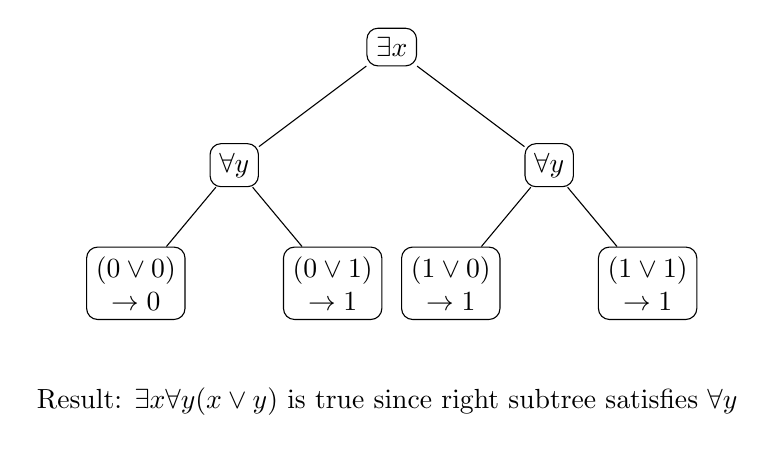
\begin{tikzpicture}[
    level distance=1.5cm,
    level 1/.style={sibling distance=4cm},
    level 2/.style={sibling distance=2.5cm},
    every node/.style={draw, rounded corners, align=center}]
  
  \node {$\exists x$}
    child {
        node {$\forall y$}
        child {node[rectangle] {$(0 \lor 0)$\\$\rightarrow 0$}}
        child {node[rectangle] {$(0 \lor 1)$\\$\rightarrow 1$}}}
    child {
        node {$\forall y$}
        child {node[rectangle] {$(1 \lor 0)$\\$\rightarrow 1$}}
        child {node[rectangle] {$(1 \lor 1)$\\$\rightarrow 1$}}};
  
  \node[draw=none] at (0,-4.5) {
    Result: $\exists x\forall y(x\lor y)$ is true since right subtree satisfies $\forall y$
  };
\end{tikzpicture}
\end{center}

\subsection{Space Efficiency}

Key observations about the algorithm:
\begin{itemize}
    \item \textbf{Depth-first evaluation}: Only one path active at any time
    \item \textbf{Space reuse}: Each completed subtree's space is reclaimed
    \item \textbf{Constant overhead}: Per recursive call uses $O(1)$ space
    \item \textbf{Total space}: $O(n)$ for $n$ variables
\end{itemize}

This shows how \texttt{TQBF} can be in \texttt{PSPACE} despite the exponential recursion tree.

    
\section{The Ladder Problem}

\begin{definition}[Ladder Problem]
The \emph{Ladder Problem} refers to the question: \emph{Given two space bounds $f(n)$ and $g(n)$ where $f(n) = o(g(n))$, does it hold that $\mathbf{SPACE}(f(n)) \subsetneq \mathbf{SPACE}(g(n))$?}

In other words, are there problems that require strictly more space than $f(n)$, but can be solved within $g(n)$ space?
\end{definition}

\begin{theorem}[Space Hierarchy Theorem (Ladder Theorem)]
Let $f(n)$ be a space-constructible function. Then there exists a language $L$ such that:
\[
L \in \mathbf{SPACE}(f(n)) \setminus \bigcup_{g(n) = o(f(n))} \mathbf{SPACE}(g(n)).
\]
That is, $\mathbf{SPACE}(o(f(n))) \subsetneq \mathbf{SPACE}(f(n))$.
\end{theorem}

\begin{proof}
The proof uses diagonalization. We construct a language $L$ that cannot be computed in space $o(f(n))$, but can be computed in $O(f(n))$ space.

Let $f(n)$ be a space-constructible function. This means we can design a Turing machine that, on input $1^n$, uses exactly $f(n)$ space.

We construct a language $L$ that "diagonalizes" against all Turing machines $M_1, M_2, M_3, \dots$ that run in $o(f(n))$ space.

On input $x$, the machine $D$ (deciding $L$) proceeds as follows:
\begin{enumerate}
    \item Compute $f(|x|)$ (possible due to space-constructibility).
    \item Simulate $M_{\#(x)}$ on input $x$, where $\#(x)$ is the Gödel number of $x$.
    \item If $M_{\#(x)}(x)$ accepts within $f(|x|)$ space, then $D$ rejects; otherwise, $D$ accepts.
\end{enumerate}

This construction ensures that $L$ differs from each $M_i$ on at least one input—specifically, its own index. Thus, $L$ cannot be decided by any machine running in $o(f(n))$ space.

\paragraph{Space Used:} All of the above can be implemented within $O(f(n))$ space: computing $f(n)$, simulating a machine up to $f(n)$ space, and inverting its result.

Hence, $L \in \mathbf{SPACE}(f(n))$ but $L \notin \mathbf{SPACE}(o(f(n)))$.

\end{proof}

\begin{remark}
This theorem justifies the term ``ladder'' because space complexity classes form a proper hierarchy as we increase the available space. That is:
\[
\mathbf{SPACE}(\log n) \subsetneq \mathbf{SPACE}(n) \subsetneq \mathbf{SPACE}(n^2) \subsetneq \dots
\]
as long as the space bounds are space-constructible and differ asymptotically.
\end{remark}

\section{Savitch's Theorem}

\begin{theorem}[Savitch's Theorem]
For any function $f(n) \geq \log n$ that is space-constructible,
\[
\texttt{NSPACE}(f(n)) \subseteq \texttt{DSPACE}(f(n)^2).
\]
\end{theorem}

\begin{remark}
Savitch's Theorem shows that nondeterministic space is not much more powerful than deterministic space. In particular, it implies that:
\[
\texttt{PSPACE} = \texttt{NPSPACE}.
\]
This is in stark contrast with time complexity, where it is widely conjectured that $\texttt{P} \ne \texttt{NP}$.
\end{remark}

\begin{proof}
We describe a deterministic algorithm that simulates a nondeterministic Turing machine (NTM) using only $O(f(n)^2)$ space.

Let $M$ be a nondeterministic Turing machine that operates in $f(n)$ space on input $x$ of length $n$. Let $C_1$ and $C_2$ be two configurations of $M$ on input $x$.

We define a recursive procedure:
\[
\texttt{REACH}(C_1, C_2, t)
\]
which returns true if there is a computation path from $C_1$ to $C_2$ in at most $t$ steps.

\paragraph{Base Case:} If $t = 1$, return true iff $C_2$ is directly reachable from $C_1$ in one step.

\paragraph{Recursive Case:} If $t > 1$, we guess a middle configuration $C_m$ and check:
\[
\texttt{REACH}(C_1, C_m, \lfloor t/2 \rfloor) \text{ and } \texttt{REACH}(C_m, C_2, \lceil t/2 \rceil)
\]
We try all possible $C_m$. The total number of configurations is at most $2^{O(f(n))}$ since each configuration uses at most $f(n)$ space.

\paragraph{Space Analysis:}
\begin{itemize}
    \item Each recursive call stores $C_1$, $C_2$, $t$, and the guessed $C_m$, requiring $O(f(n))$ space per call.
    \item The recursion depth is $O(\log t)$, and $t \leq 2^{O(f(n))}$.
    \item Therefore, total space is $O(f(n) \cdot \log t) = O(f(n)^2)$.
\end{itemize}

Thus, a deterministic Turing machine can simulate the NTM using $O(f(n)^2)$ space.
\end{proof}

\begin{remark}
The key insight is that while time is inherently sequential and expensive to simulate deterministically, space can be reused. Savitch's algorithm uses divide-and-conquer to recursively check for reachability in the configuration graph of the machine.
\end{remark}


\section{The Classes \textsf{L} and \textsf{NL}}

\subsection{Definitions}

\begin{definition}[Logarithmic Space Complexity]
Let $M$ be a Turing machine with:
\begin{itemize}
    \item A read-only input tape
    \item A read/write work tape
    \item (For nondeterministic machines) A read-once witness tape
\end{itemize}
We say $M$ operates in \emph{logarithmic space} if it uses at most $O(\log n)$ cells on its work tape(s) for inputs of size $n$.
\end{definition}

\begin{definition}[The Class \textsf{L}]
\textsf{L} is the class of languages decidable by deterministic Turing machines in logarithmic space.
\end{definition}

\begin{definition}[The Class \textsf{NL}]
\textsf{NL} is the class of languages decidable by nondeterministic Turing machines in logarithmic space.
\end{definition}

\subsection{Key Results}

\begin{theorem}[Basic Relationships]
The logarithmic space classes satisfy:
\[
\textsf{L} \subseteq \textsf{NL} \subseteq \textsf{P} \subseteq \textsf{NP}
\]
\end{theorem}

\begin{theorem}[Immerman-Szelepcsényi]
\textsf{NL} = \textsf{coNL}, demonstrating that nondeterministic logarithmic space is closed under complement.
\end{theorem}

\subsection{Complete Problems}

\begin{itemize}
    \item \textsf{L}-complete: 
    \begin{itemize}
        \item Undirected $s$-$t$ connectivity (USTCON)
        \item Deterministic acyclic automaton emptiness
    \end{itemize}
    
    \item \textsf{NL}-complete:
    \begin{itemize}
        \item Directed $s$-$t$ connectivity (STCON)
        \item 2SAT (satisfiability of 2-CNF formulas)
    \end{itemize}
\end{itemize}

\subsection{Algorithmic Techniques}

\begin{example}[Reachability in \textsf{NL}]
The STCON problem can be solved by:
\begin{algorithmic}[1]
\STATE Initialize $c \gets s$ (current vertex)
\FOR{$i \gets 1$ to $n$}
\STATE Nondeterministically choose neighbor $v$ of $c$
\STATE $c \gets v$
\IF{$c = t$} \RETURN true \ENDIF
\ENDFOR
\RETURN false
\end{algorithmic}
This uses $O(\log n)$ space to track the current vertex.
\end{example}

\subsection{Open Problems}

\begin{itemize}
    \item Does \textsf{L} = \textsf{NL}? (Widely believed to be false)
    \item Is \textsf{NL} = \textsf{P}? (Related to whether we can derandomize space-bounded computation)
\end{itemize}

